\documentclass{article}

% Packages
\usepackage{cite}
\usepackage[pdftex]{graphicx}
\usepackage[utf8]{inputenc}
\usepackage[english]{babel}
\usepackage{indentfirst}
\usepackage{fancyhdr}
\usepackage{tikz}
\usepackage[a4paper, headheight=14pt, total={7.37in, 8in}]{geometry}

% Settings
\setlength{\parskip}{1em}
\setlength{\parindent}{4em}

% Commands
\newcommand{\HRule}{\rule{\linewidth}{0.5 mm}}
\newcommand*\circled[1]{\tikz[baseline=(char.base)]{
            \node[shape=circle,draw,inner sep=2pt] (char) {#1};}}

\begin{document}
\begin{titlepage}
\begin{center}


\includegraphics[width=0.15\textwidth]{img/logo}~\\[1 cm]

\textsc{\LARGE University of Utah}\\[1.5 cm]

\textsc{\Large Madadasa}\\[1.5 cm]

% Title
\HRule \\[0.4 cm]
{  \huge \bfseries Principia: Design Document
	\\[0.4 cm]}

\HRule \\[1.5 cm]

%Author and Supervisor
% Author and supervisor
\noindent
\begin{minipage}{0.4\textwidth}
\begin{flushleft} \large
\emph{Authors:}\\
Sam \textsc{Olds}\\
Daniel \textsc{Peterson}\\
Matthew \textsc{Turner} \\
Dalton \textsc{Wallace}\\
\end{flushleft}
\end{minipage}%
\begin{minipage}{0.4\textwidth}
\begin{flushright} \large
\emph{Supervisor:} \\
H. James \\ \textsc{de St. Germain}
\end{flushright}
\end{minipage}

\vfill

% Bottom of the page
{\large \today}

\end{center}
\end{titlepage}

% page 1
\thispagestyle{fancy}
\fancyhf{}
\lhead{Principia}
\rhead{Madadasa}
\rfoot{\circled{\thepage}}

% EXECUTIVE SUMMARY:
\section{Executive Summary}
\iffalse
The purpose of this introduction to your idea is to clearly and succinctly describe the final goal of the project. It should list key features and components and explain why the project is interesting and worthwhile.

When "searching for funding/approval" you have very little time/space to capture the interest of the reader. You need to concisely describe what the project will do, what need it will address, and why a completed project with be of benefit. You also need to convey interest, enthusiasm, and determination. You want the reader coming away from this first page eager to know more and excited about the prospects.
 
This section should be one page long.

NOTES:
Look at: 
"A meta-analysis of the effectiveness of computer-assisted instruction in science education"

"Success in introductory college physics: the role of high school preparation"

"STEM Attrition: College Students' Paths Into and Out of STEM Fields"

"Trends in International Mathematics and Science Study"

\fi

Physics is one of the core subjects that college-bound high school students will explore, especially for those that plan on pursuing a degree in a scientific field. However, many instructors have their doubts about how well high school courses are preparing students for their college experience. According to a 2013 study by U.S. Department of Education, 46\% of beginning bachelor's degree students in the physical sciences either left their post-secondary education without a degree or changed majors. For those beginning an associates degree, 64\% of such students did the same. %Stem attrition%
% Also find statistics on dropout rates here, TIMSS could be useful
% Statistics on the benefits of using software in education?
% First study I found indicates it makes little difference...

Clearly, there is a need for improvement in this area. Our team believes that we can provide a web-based solution that would have the power to make a difference for both high school students and students taking college level physics for the first time. Our project will be called \textit{Principia}, named after \textit{Philosophiæ Naturalis Principia Mathematica}, the collection of books written by Newton that serve as the foundation of classical mechanics. 

We envision Principia as a website that is in equal parts an engaging community experience and a powerful tool to model physical systems. Students will have a support network that will help them overcome challenges and a chance to share their knowledge with others.

The core feature will be an interactive sandbox for designing systems. It will include a toolbox that contains components like point masses, springs, and pulleys. Users can drag and drop these components into a central canvas. Within the canvas, any instance of a component can be selected and its properties will be displayed on the side of the window. See section x for an enumeration of the components we will support and section y for figures demonstrating our plans for the UI. 

Once the components are in place, users can select play and the canvas will come to life. The components will move over time according to their properties, allowing students to visualize the system. At any point, they can pause the simulation and select a component to view its properties, allowing them to get quantitative results in addition to the visualization. 

Principia will feature much more than the sandbox. To enable users to connect with and support one another, the website will support the creation of accounts with additional features. A registered user can save and load their creations, share them with others, browse simulations, provide comments and annotations, and even create quizzes and walkthroughs. Imagine a future where instructors integrate Principia into their course. No longer will students work in isolation, writing out equations based on a static image or an ambiguously worded problem. Instead, students will have the chance to engage with both the instructor and their peers, exploring problems interactively or even inventing their own systems.

% Replace fantastic with a better word
We see the final version of Principia as potentially being the number one site for physics education as a fantastic supplement to any physics classroom as well as a tool that empowers motivated individuals to educate themselves with the support of a community.
% ---

% page2
\newpage
\thispagestyle{fancy}
\fancyhf{}
\lhead{Principia}
\rhead{Madadasa}
\rfoot{\circled{\thepage}}

% BACKGROUND:
\section{Background}
\iffalse
The background section should be one to three pages long.
\fi

% ----------------- Idea Space -----------------
\subsection{Idea Space}
\iffalse
Why is your project needed? What problems does it solve? Who would use it?
\fi
\BgThispage
We believe that the most memorable physics lessons were the ones with demonstrations. The best lecturers came to class with props and experiments used to reinforce the lesson's material. However, students don't always have the means to recreate the demonstrations to get a better understanding of the underlying concepts. Furthermore, not every instructor has the resources or time to prepare practical demos.

Principia would solve both of these problems. Students would be able to easily build their own simulations of the in-class demonstrations and tweak components to see how their changes affect the end result. This would make learning physics more visual and interactive, and ultimately more fun! Instructors would also be able to share simulations, eliminating the need to purchase special equipment or to spend precious class time setting up an experiment. 

The fundamental problem we wish to address, however, is the poor state of physics education itself. Dr. John W. Brelsford studied the effects of virtual reality specifically within the context of physics education. His found that ``As a training method, virtual reality was superior to the [lecture-based] control condition at the four-week retention period. Such a finding supports cognitive theorists who argue that the lack of opportunities for hands-on, manipulation of objects in the physical world is one of the reasons children are often poor at intuitive physics. Virtual reality provides them the opportunity to develop manipulational skills they did not previously possess'' \cite{Brelsford}.

Principia's sandbox is precisely the kind of tool that improved physics knowledge retention in Dr. Brelsford's study. The addition of support from an online community will make for even better software. Principia will improve the state of physics education on a worldwide scale.

%A user can build a system by dragging and dropping elements like ramps, pulleys, or springs into a frame in their browser. Then the simulation can be run to see the elements interact with each other over time, with the ability to pause the simulation at any point and query the state of an element. Users can save their simulations and share them with others in the community. Special privileges are available for instructor accounts to manage a classroom, including the ability to incorporate quizzes or assignments into their physics system.

% ----------------- Similar Ideas -----------------
\subsection{Similar Ideas}
\iffalse
List and describe other programs that do things like what you want to do. Why is your idea different or better?
\fi
\noindent
While we assert that there is significant room for innovation and improvement in the area of physics education, we acknowledge several existing educational offerings.


\subsubsection{Commercial Software}
There is a wide array of commercial software for physics. Some are focused on a very specific domain for professionals, such as molecular dynamics or high-energy physics. This kind of software would not be useful to the audience we are targeting. Other examples that do focus on high school or college physics, like Stewart Software's Creative Physics\textup{\textregistered} 5.0, cost as much as \$149.99 for a single-user license \cite{CreativePhysics}. We want to provide software that has a lower barrier for entry and that puts improving the state of physics education above financial gain.

\subsubsection{Physion}
Physion is the closest existing software to what we want to provide. It is highly interactive, free, and has a modest online community. However, we believe we can improve on it by having Principia's sandbox run in-browser instead of as a separately downloaded executable and by providing greater support for getting quantitative data out of the simulation.

\clearpage
\BgThispage
\subsubsection{smartPhysics}
Arguably the most prominent offering on the current market,  smartPhysics provides students with additional examples and resources to help solidify concepts learned in the classroom. This is primarily accomplished through online ``pre-lectures'' and homework material.  In our experience with smartPhysics, we have found that it lacks interactivity, relegating users to working on practice problems involving systems that the smartPhysics developers have already created. For instance, the following figure is a sample image of a checkpoint concerning simple harmonic motion. This checkpoint will always involve a single spring attached to a single mass. The practice problem can be varied by adjusting the values associated with the amount of mass or the spring constant, but there is no way to see the system in motion or to experiment with how additional components like a second spring or surface friction would affect its behavior.

smartPhysics is a great way of introducing concepts, but it is possible to do much more. Our goal with Principia is to provide a new level of interactivity, allowing a user to explore concepts and ideas specific to her needs by building her own systems or modifying existing ones rather than being limited to ``canned'' systems as in this example.

\begin{figure}[H]
	\centering
	\fbox{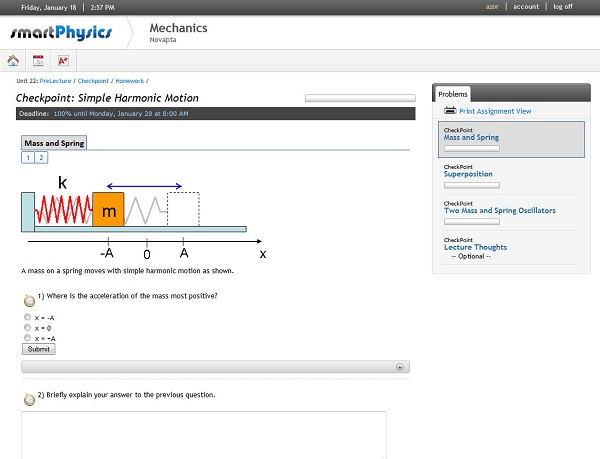
\includegraphics[scale=0.6]{img/SmartPhysics}}
    \caption{Smart Physics checkpoint \cite{smartPhysics}}
\end{figure}

\subsubsection{PhET}

PhET is an open-source collaboration developed by a group of researchers from UC Boulder. The project aims to provide ``fun, free, interactive, research-based science and mathematics simulations''.  While PhET offers a measure of interactivity, the number of physics topics it covers is relatively limited. It is more dynamic than smartPhysics, as should be apparent in the following figure, but it is still limited by the fact that users are tweaking the properties of an existing system instead of building their own in a less restrictive environment.

\clearpage
\BgThispage


\begin{figure}[H]
	\centering
	\fbox{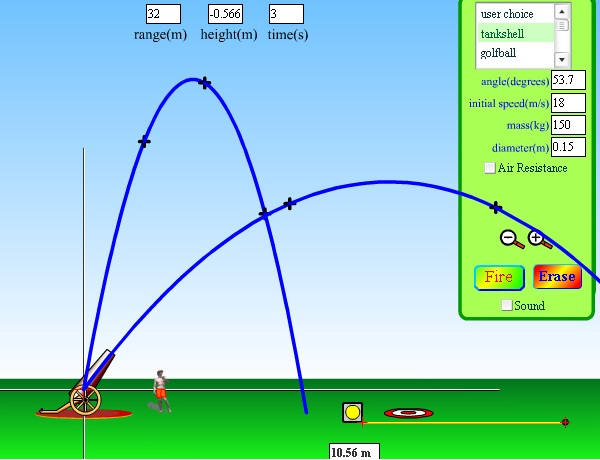
\includegraphics[scale=0.55]{img/phet}}
    \caption{Projectile motion in PhET \cite{PhET}}
\end{figure}

\subsubsection{WebAssign}

WebAssign allows educators to set up online environments designed to test student knowledge and offer additional instruction.  Principia would expand upon this idea by not only providing an environment for instructors to engage their students but also allow students to query their classmates with specific questions and concerns.  In addition, we feel that Principia would provide more freedom when creating quizzes or exams.  For example, with Principia teachers could pose questions that would require students to modify a specific portion of a simulation and explain how their change affected the simulation's outcome.  

\begin{figure}[H]
	\centering
	\fbox{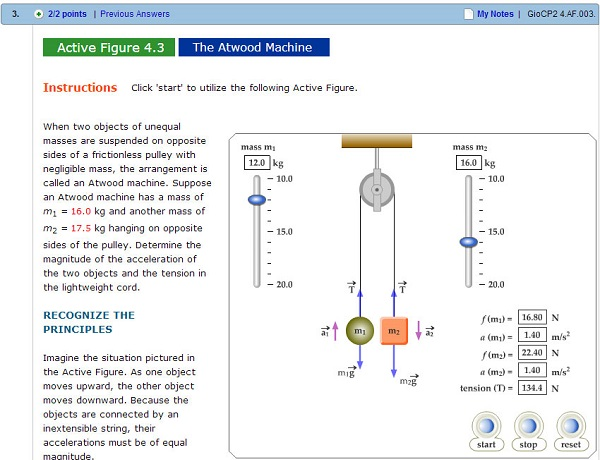
\includegraphics[scale=0.55]{img/WebAssign}}
    \caption{Active figure in WebAssign \cite{WebAssign}}
\end{figure}



\clearpage
\BgThispage
% ----------------- Required Technology -----------------
\subsection{Required Technology}
\iffalse
List and describe the software technologies that you will either need to implement or utilize to realize your project goals.
\fi
\noindent
Principia will require the following technologies:
\begin{itemize}
\item A web server where the application can be hosted.
\item A database to hold information about users and their saved simulations.
\item A simulation window nested in an HTML page that allows for interactivity.
\item A physics engine that will accurately update the simulator's physics model and render the results.
\end{itemize}

% ----------------- Assets and Engines -----------------
\subsection{Assets and Engines}
\iffalse
How much will you be building from scratch? What resources/assets will you leverage? Where will they come from?
\fi
\noindent
To avoid rebuilding the wheel for every component, we will be using the following languages, services, and libraries:
\begin{itemize}
\item Go will be the language used on the server and back end.
\item Google App Engine will be used to host the web application.
\item HTML, CSS, and JavaScript will all be languages used on the front end.
\item The HTML {\textless}canvas{\textgreater} element will be used for the simulator window.
\item To help with some of the difficult physics components, we will utilize the open source JavaScript library, PhysicsJS. It has in-built support for rendering into an HTML canvas and will allow us to write high-level code for the physics model instead of creating it from scratch.
\item To help provide a consistent theme and feel across browsers, Twitter's Bootstrap CSS library will be used.
\item AngularJS will be used to make the front end more user friendly and responsive.
\end{itemize}

% ----------------- Software Requirements -----------------
\subsection{Software Requirements}
\iffalse
List and describe what hardware and/or software you will need to successfully install and use your software.
\fi

In order to fully use Principia, the user will need a computer with access to the Internet and a web browser. We plan to support all of the mainstream browsers, including Google Chrome, Safari, Mozilla Firefox, and Internet Explorer. Since it is a web application, the site will be available on mobile devices; however, we don't plan to explicitly support mobile devices. We will make a ``best-effort'' approach analogous to ``best-effort'' packet delivery, i.e. we make no functional guarantees! No separate download or special hardware will be required to use the simulator. It will be easier to build a community around our project if it has a low barrier for entry.
% ---

\end{document}